\section{Cronograma e Fluxo de Atividades}\label{cronograma}

\subsection{Atividades da Primeira Etapa}
\label{cronograma1}


Esta subseção visa discriminar as atividades realizadas na primeira etapa do trabalho, os apresentando também em forma de fluxo na Figura \ref{fig:atividades_1} e às dispondo cronologicamente na Figura \ref{fig:cronograma_1}.

\begin{figure}[h!]
    \caption{Fluxo de Atividades Realizadas na Primeira Etapa Desta Monografia}
    \centering
    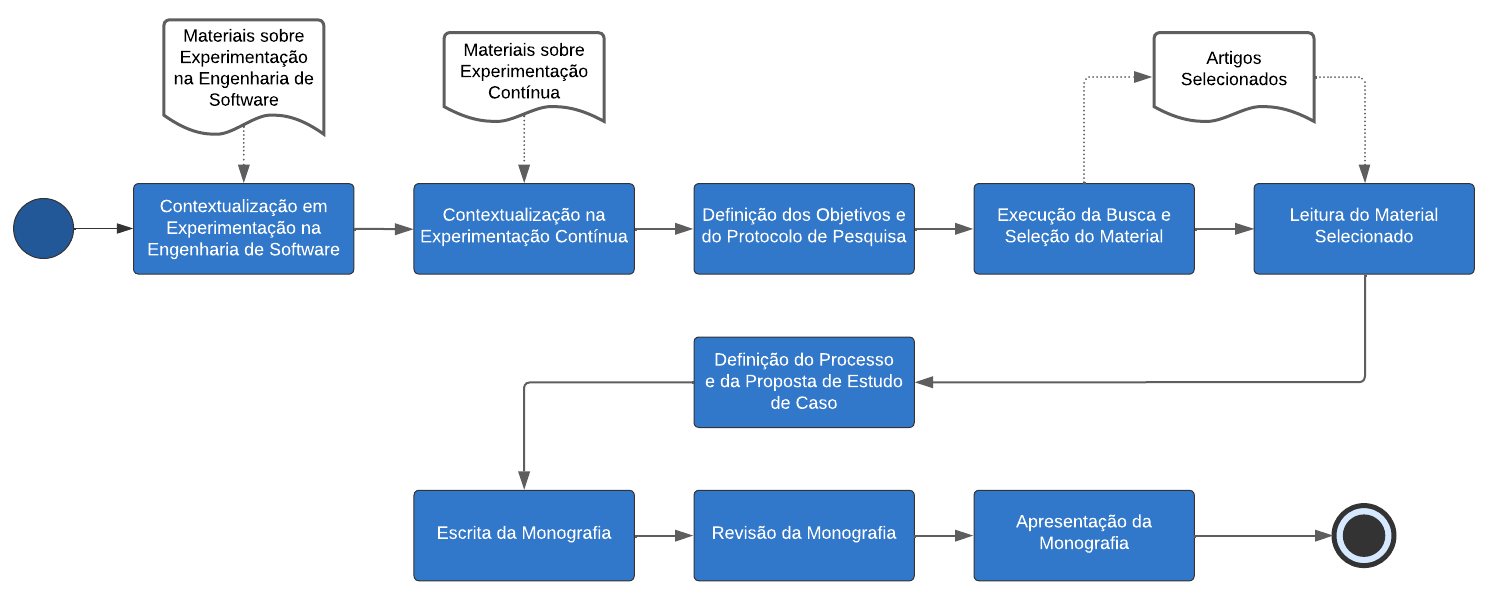
\includegraphics[width=.9\linewidth]{figuras/atividades1.png}
    \text{Fonte: Autor}
    \label{fig:atividades_1}
\end{figure}

\begin{figure}[h!]
    \caption{Cronograma Realizado na Primeira Etapa da Monografia}
    \centering
    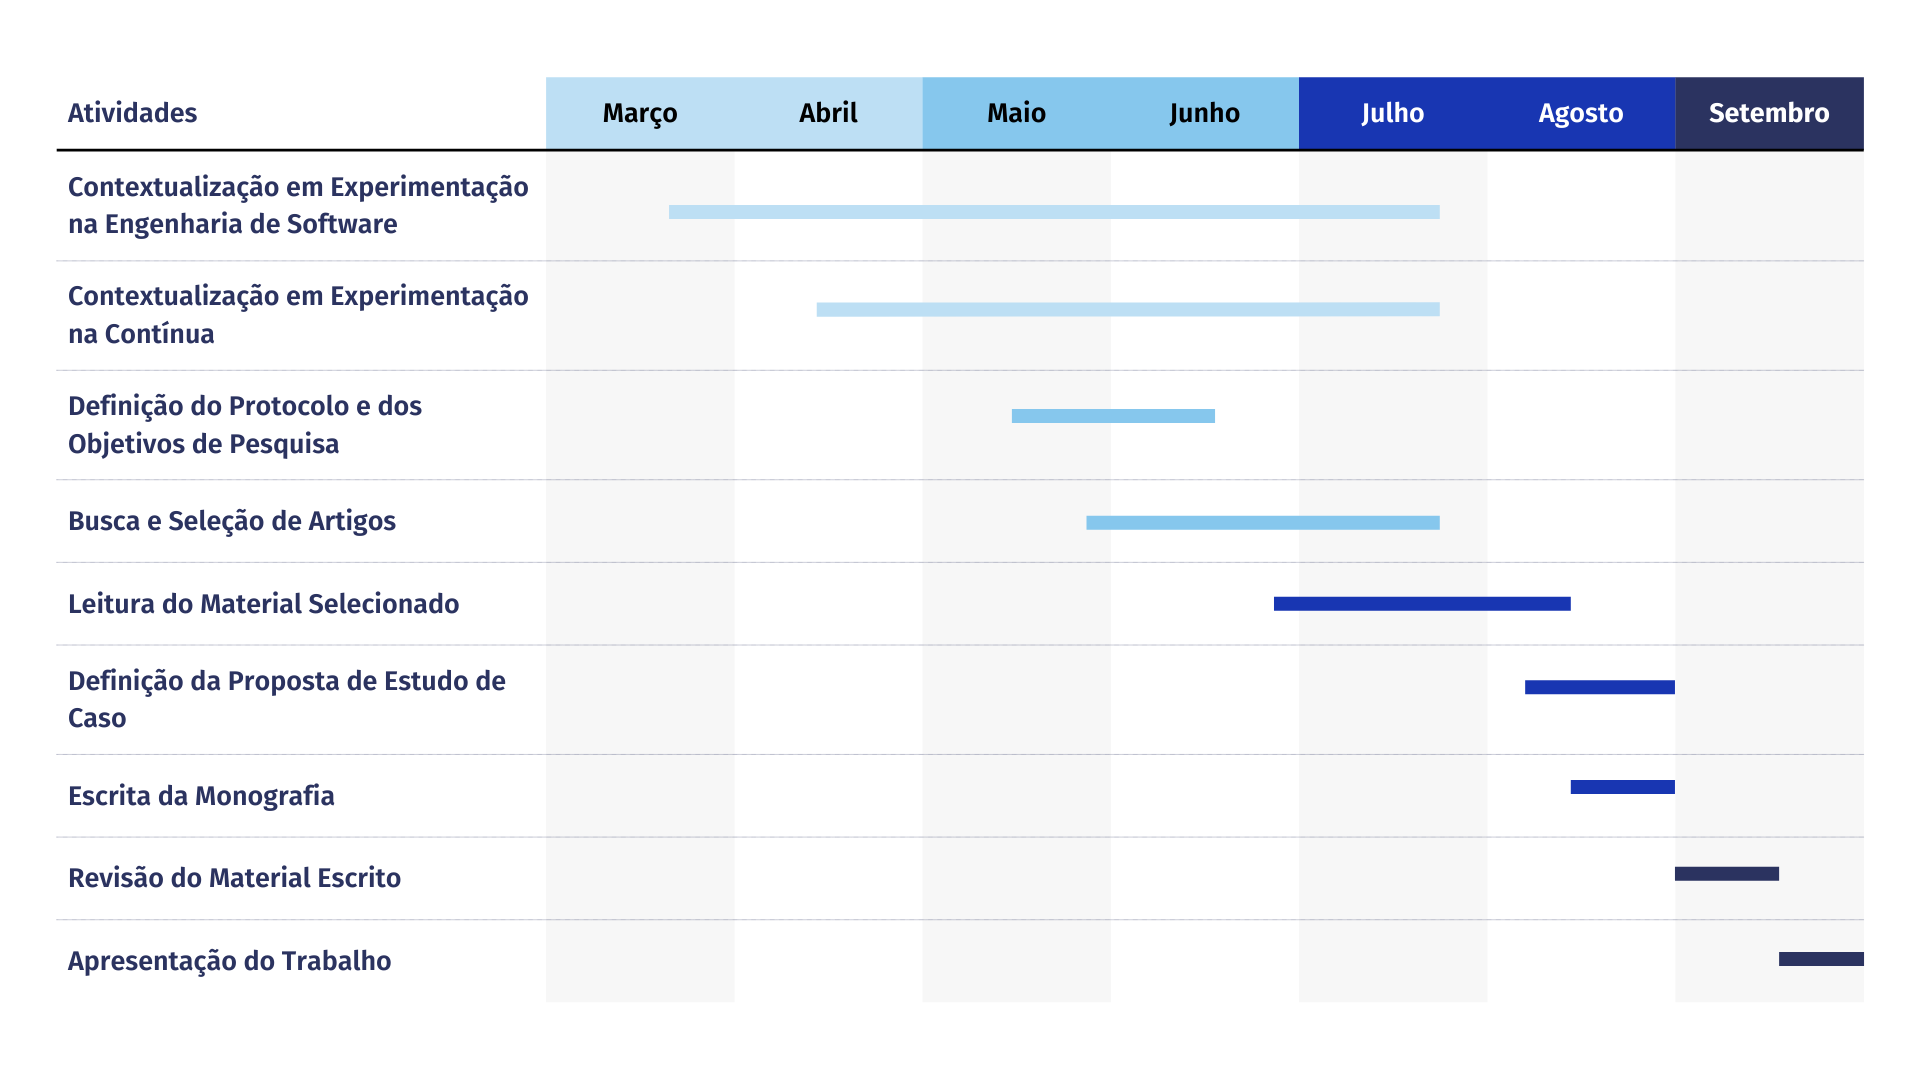
\includegraphics[width=.9\linewidth]{figuras/cronograma1.png}
    \text{Fonte: Autor}
    \label{fig:cronograma_1}
\end{figure}


\begin{itemize}
    \item \textbf{Contextualização em Experimentação na Engenharia de Software:} leituras com o intuito de compreender o processo de experimentação e a abordagem científica necessária para a realização da Revisão da Literatura da primeira parte desta pesquisa, em como do Estudo de Caso, e do Experimento que serão realizados na segunda parte;
    \item \textbf{Contextualização em Experimentação Contínua:} leitura de materiais referentes ao processo de Experimentação Contínua e Desenvolvimento Orientado a Dados com o objetivo de compreender o estado da arte, identificar as lacunas existentes e moldar os objetivos deste trabalho; consumo de materiais para capacitação do pesquisador nas áreas de qualidade de software e experimentos científicos;
    \item \textbf{Definição dos Objetivos e Protocolo de Pesquisa:} definição do protocolo de revisão da literatura e dos objetivos da pesquisa segundo a abordagem GQM \cite{basili_goal_1994}, além dos objetivos específicos e da questão de pesquisa do trabalho; formulação do protocolo de pesquisa conforme proposto por \citeonline{kitchenham_rsl}: questões de pesquisa da revisão, \textit{string} de busca, critérios de inclusão e exclusão e formulário de extração de dados;
    \item \textbf{Busca e Seleção dos Artigos:} execução da \textit{string} de busca e seleção do primeiro grupo de artigos a partir da leitura de título e resumo; processo de \textit{snowballing} a partir dos artigos selecionados, selecionando novos materiais a partir da leitura parcial dos mesmos (título e resumo e, caso necessário, introdução e conclusão);
    \item \textbf{Leitura do Material Selecionado:} leitura integral do material selecionado com o objetivo de compreender o estado da arte, conhecer os modelos e processos já existentes e construir o corpo de conhecimento necessário para a formulação da proposta de estudo de caso;
    \item \textbf{Definição da Proposta de Processo:} elaboração da proposta de processo de experimentação; formalização da proposta de estudo de caso, discriminando objetivos, objeto, instrumentalização e atividades a serem realizadas;
    \item \textbf{Escrita do Trabalho:} redação da monografia seguindo a organização apresentada na Seção \ref{sec:organizacao};
    \item \textbf{Revisão da Monografia:} revisão e correção; e
    \item \textbf{Apresentação do Trabalho:} apresentação da primeira parte desta monografia para a banca avaliadora.
\end{itemize}


\subsection{Atividades da Segunda Etapa}
\label{cronograma2}

Esta subseção visa apresentar as atividades planejadas para a segunda etapa deste trabalho,
as apresentando em forma de fluxo na Figura \ref{fig:atividades_2} e as dispondo em forma de cronograma na Figura \ref{fig:cronograma_2}.

\newpage

\begin{figure}[h!]
    \caption{Fluxo de Atividades Planejadas Para a Segunda Etapa da Monografia}
    \centering
    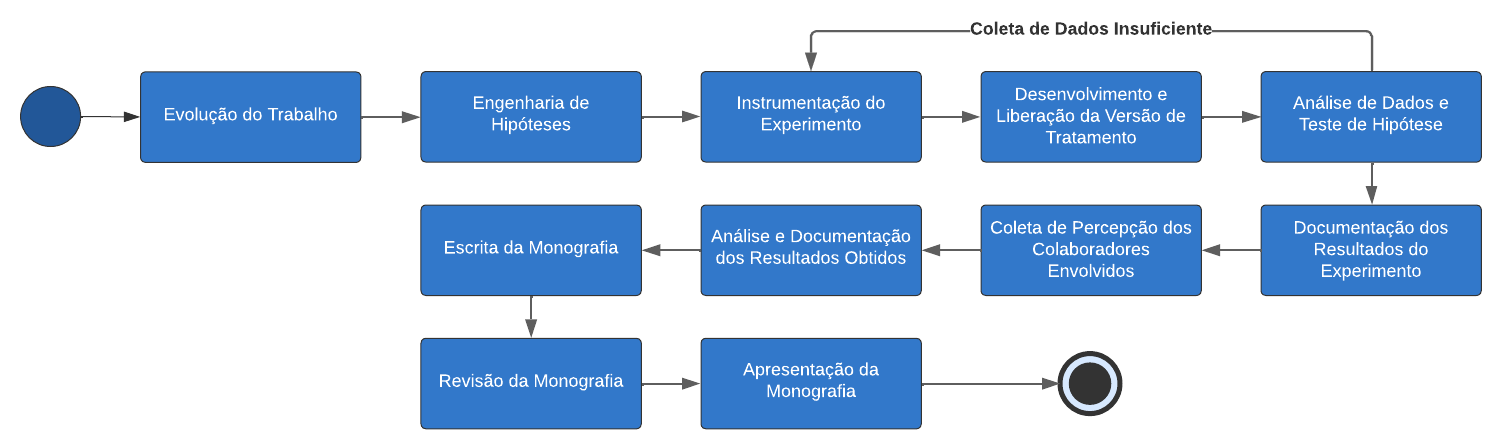
\includegraphics[width=.9\linewidth]{figuras/atividades2.png}
    \text{Fonte: Autor}
    \label{fig:atividades_2}
\end{figure}

\begin{figure}[h!]
    \caption{Cronograma Planejado Para a Segunda Etapa da Monografia}
    \centering
    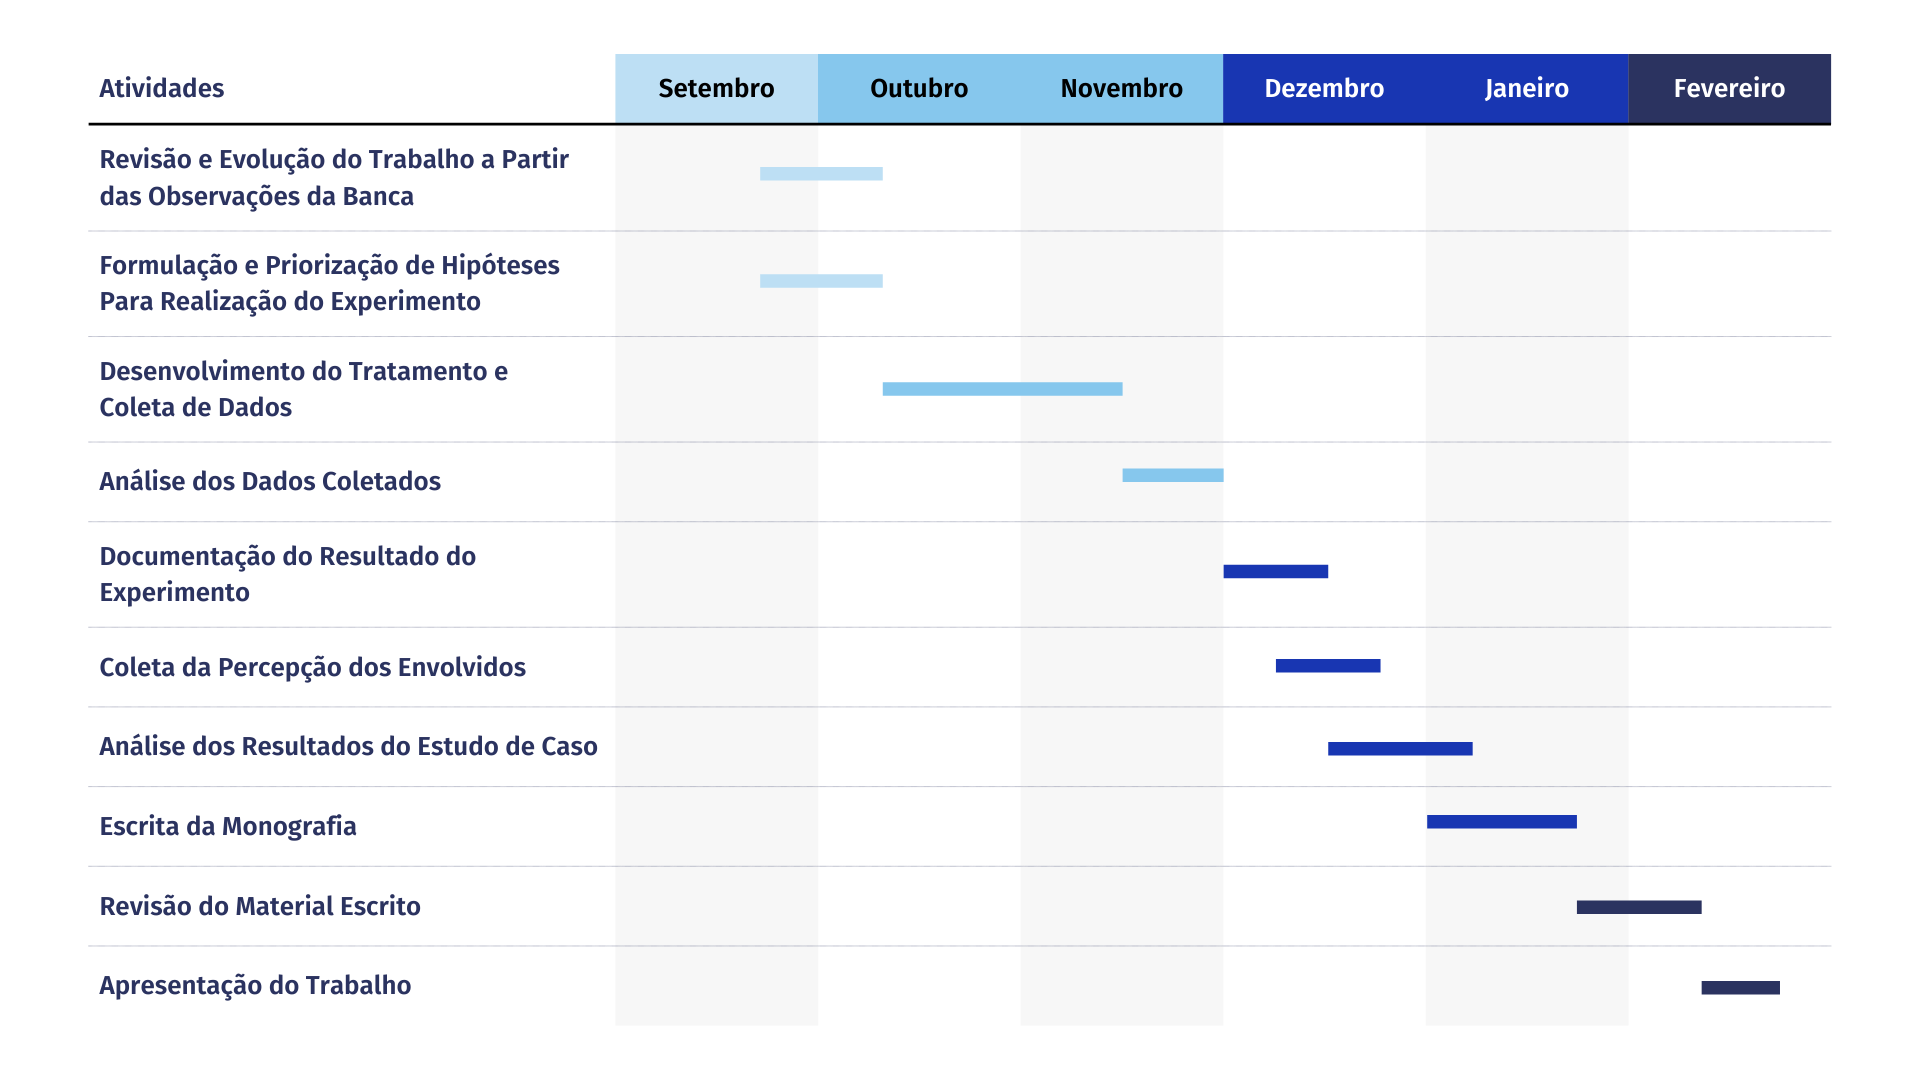
\includegraphics[width=.9\linewidth]{figuras/cronograma2.png}
    \text{Fonte: Autor}
    \label{fig:cronograma_2}
\end{figure}


\begin{itemize}
    \item \textbf{Evolução do Trabalho:} revisão e atualização do material já escrito a partir das considerações da banca avaliadora;
    \item \textbf{Formulação de Hipóteses:} realização das atividades referentes à Engenharia de Hipóteses; geração, documentação e priorização de hipóteses para escolher aquela que será desenvolvida e observada através da execução do experimento objeto do Estudo de Caso deste trabalho;
    \item \textbf{Instrumentação do Experimento:} prototipação da hipótese selecionada; definição das métricas escolhidas para validação da hipótese; preparo dos disparos de evento para coleta dos dados; validação do \textit{design do experimento}; revisão da hipótese ou das métricas elencadas, caso necessário;
    \item \textbf{Desenvolvimento e Coleta de Dados:} desenvolvimento da nova versão de software (tratamento) a ser comparada com a versão já existente (controle); liberação da nova versão para os usuários beta a fim de iniciar a iteração do experimento (a coleta de dados já deve acontecer a partir desta liberação);
    \item \textbf{Análise de Dados:} iteração no experimento caso necessário (como, por exemplo, dados coletados insuficientes, necessidade de prolongamento do experimento); análise dos dados coletados para os testes de hipótese; decisão sobre a liberação da versão de tratamento para todos os usuários ou abandono da mesma;
    \item \textbf{Documentação do Resultado do Experimento:} documentação dos resultados do teste da hipótese para registro e criação de um corpo de conhecimento que auxilie futuros experimentos;
    \item \textbf{Coleta de Percepção dos Envolvidos:} pesquisa de opinião com os colaboradores envolvidos no estudo de caso para avaliação do processo proposto;
    \item \textbf{Análise dos Resultados do Estudo de Caso:} resposta às questões de pesquisa do estudo de caso a partir dos dados coletados, com posterior resposta à principal questão de pesquisa; descrição do processo realizado e documentação dos resultados obtidos;
    \item \textbf{Revisão da Monografia:} revisão e correção minuciosa do trabalho em busca de possíveis correções ou atualizações necessárias, tanto por parte do pesquisador quanto do orientador; e
    \item \textbf{Apresentação do Trabalho Finalizado:} apresentação da monografia finalizada à banca avaliadora.
\end{itemize}



